\documentclass[../main.tex]{subfiles}

\begin{document}
\section{Additional Character Info}
This section contains a more in-depth breakdown of the Character card.

\subsection{Calculating Stats}
There are several different ways in which a Character’s stats may be modified. When using a Character’s stat, always use their Total Stat, which can be calculated by performing the following steps:

\begin{enumerate}
    \item Check your Character's Base Stat.
    \item Check to see if there are any Awakened, buff, or curse modifiers showing in that stat's row. 
    \item If using a skill, check to see if the skill modifies the stat. 
    \item If the Character has an artifact equipped, check to see if the artifact modifies the stat. 
    \item Add together the values from steps 1- 4 to determine the Character's Total Stat. 
\end{enumerate}

\textit{A Character with the Movement buff has a base Movement stat of 5 and their Movement buff is active showing +2. Add two to the Base Stat for Movement, resulting in a total Movement of 7.}

\subsection{Buffs and Curses}
Buff and curse stat modifiers can be gained by and removed from Characters throughout the game. When a buff or curse is gained by a Character, the marker is removed from the slot for that buff or curse. When a buff or curse is removed from a Character, the marker is placed back in the corresponding slot. Buffs typically increase stats and add new beneficial effects to the Character. Curses typically decrease stats and add detrimental effects to the Character. Buffs and curses can be applied to Characters through skills or other events. 

\centering
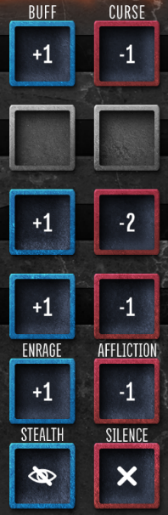
\includegraphics[width=0.25\linewidth]{chapters//AdditionalCharacterInfo/TimeStrikeBuffsandCursesGraphic.png}

\textit{Note: If a Character has both a buff and curse applied to the same stat, (Move, Range, Attack, or Defense) the buff and curse cancel each other out completely, regardless of their values.}

\textit{Example: If a Character has the Movement buff but then receives the Movement curse, this results in the Character applying no modifiers to its Movement stat from the Movement curse or buff.}

\subsection{Buffs}
The Movement, Range, Attack, and Defense buffs only change the Total Stats of the Character. There are also two other types of buffs that have unique effects.

\subsubsection{Stealth}
Units with the Stealth buff active cannot be selected as the target of attacks from units that they are not engaged with. They can still be targeted and attacked by units they are engaged with or hit by area of effect damage. Taking any damage immediately removes the Stealth buff. 

\subsubsection{Enrage}
Whenever a unit with the Enrage buff Attacks or Defends, that unit may use the buff to add the number of dice listed in the Enrage buff box to that attack or defense roll. After the Enrage buff is used, the buff is immediately removed.

\textit{Note: When Enrage is used on a Multi-unit Character, it is removed after any one unit uses it. Each unit does not get to use the Enrage.}

\subsection{Curses}
The Movement, Range, Attack, and Defense curses only change the Total Stats of the Character. There are also two other types of curses that have unique effects.

\subsubsection{Affliction}
When a Character has the Affliction curse, the Character will take the amount of damage listed on the Affliction curse at the beginning of the Character’s next turn. Once the damage is taken, the Affliction curse is immediately removed.

\textit{Note: Some Characters have a positive value on the Affliction curse; if so, the Affliction curse heals that Character instead of inflicting damage. In this case, the Affliction curse is still removed at the start of the Character’s turn even if no damage was healed.}

\subsubsection{Silence}
When a Character receives the Silence curse, the Character’s skills are reset and it is unable to use any skills until this curse is removed.

\textit{Note: Silence affects all skill types unless otherwise stated.}

\clearpage
\end{document}